\section{The modified Hilbert curve} \label{SEC_HILBERT_CURVE}

The three-dimensional modified Hilbert curve is a space-filling
curve which is used in ALG for its ability to provide an easy,
efficient and predictable way of ordering the cells of the mesh
independently of its irregularity and at the same time for having
the property of making it possible to divide the mesh in relatively
independent sub-meshes (see Figure \ref{FIG_IRREGULAR_CURVE}). Its insensitivity to the irregularity of the
mesh is mainly due to the fact that local changes in the mesh
require only local changes in the curve. This fact also accounts for
its ability to isolate different regions of the mesh. The
subdivision of the mesh into independent regions through the Hilbert
curve allows the potential use of parallel computing, since
different processes can work simultaneously on different cell
groupings.

\begin{figure}[H]
\centering
    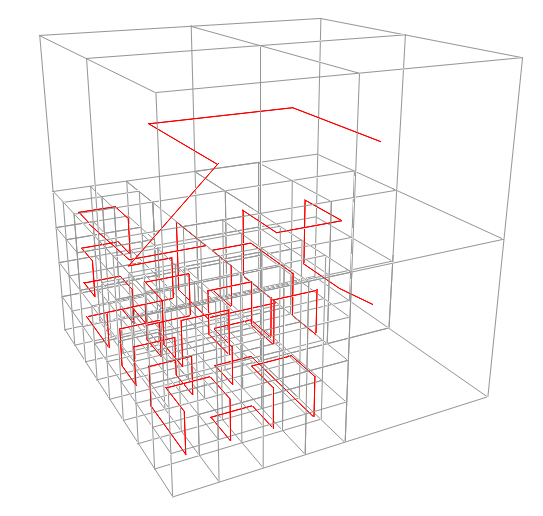
\includegraphics[scale=0.4]{../img/irregularCurve.jpg}
    \caption{Modified Hilbert curve on an irregular mesh.}
    \label{FIG_IRREGULAR_CURVE}
\end{figure}

\subsection{Implementation} \label{SUBSEC_HILBERT_CURVE_IMPLEMENTATION}

The modified Hilbert curve is implemented as a double chain list:
every cell in the mesh, besides having six directional pointers,
possesses also a pointer for the next cell and a pointer for the
previous cell. Thus any cell in the mesh can be reached by
traversing the list until it is located.

\subsubsection{The basic shapes and the Hilbert shape number}
The curve is built recursively by combining $12$ different ways of
ordering the eight cells of a bunch (see Figure
\ref{FIG_BASIC_SHAPES}). Each of these orderings is called a
\textit{basic shape} of the Hilbert curve and constitute the base
cases for the recursion. Initially, one of the basic shapes is
chosen for the ordering of the initial mesh. When one of the cells
of this initial mesh is refined, the new bunch is also ordered
according to one of the $12$ basic shapes. After the ordering, the
segment of curve in the new bunch is connected to the main curve
forming a unique continuous curve.

\begin{figure}[H]
\centering
    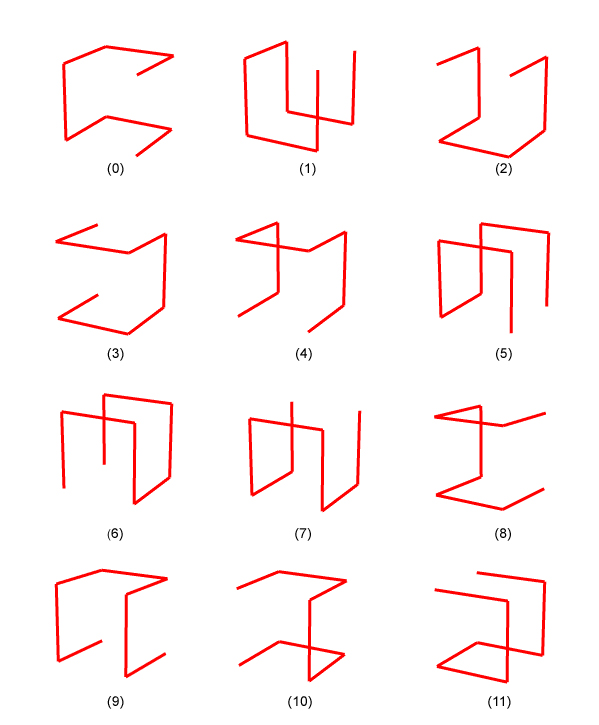
\includegraphics[scale=0.4]{../img/basicShapes.jpg}
    \caption{Basic shapes of the Hilbert curve.}
    \label{FIG_BASIC_SHAPES}
\end{figure}

Each cell in the initial graph stores the number of the basic shape
that will be used in the ordering of the cells in the new bunch in
case it is refined, which is called the \textit{Hilbert shape
number}. When a refinement occurs, the newly created bunch is always
ordered according to the basic shape informed by the refined cell.
Each of the new cells of this bunch also stores the number of the
basic shape which will be used in case the cell itself is also
refined. This way, the modified Hilbert curve is recursively defined
from the $12$ basic shapes. This process does not require the mesh
to be uniformly refined, differently from the traditional Hilbert
curve which works only on regular meshes. The modified Hilbert curve
has the advantage of supporting local changes in the mesh, when only
one cell is refined or only one bunch is derefined.

As an example of this procedure, consider the refinement of cell
number zero in Figure \ref{FIG_INITIAL_HILBERT_CURVE} (a). Upon
refinement, it will be replaced by a bunch that will be ordered
according to the Hilbert shape number stored in the original cell.
For cell zero, this was set to be number 1. After the ordering of
the bunch's cells using the basic shape 1, the main curve and the
segment of curve in the new bunch are connected, resulting in the
curve of Figure \ref{FIG_INITIAL_HILBERT_CURVE} (b).

%HILBERT INICIAL
\begin{figure}[H]
    \centering
    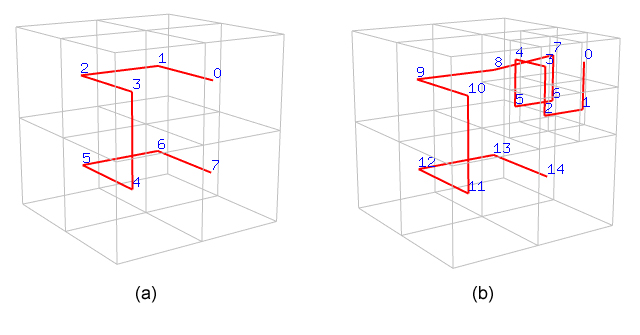
\includegraphics[scale=0.38,angle=0]{../img/initialHilbertCurve.jpg}
    \caption{Example of reordering of mesh cells using the modified Hilbert curve after the refinement of one cell.}
    \label{FIG_INITIAL_HILBERT_CURVE}
\end{figure}

In this work, the convention was made that the cells in the initial
mesh will be always ordered using the basic shape number zero of
Figure \ref{FIG_BASIC_SHAPES}. Afterwards, the way a basic shape
number is assigned to a cell in the mesh depends on the position of
the cell in its bunch and the number of the basic shape that was
used in ordering the bunch.

Table \ref{TAB_ASSIGNEMENTS_OF_BASIC_SHAPES} shows how to define the
Hilbert shape number for each cell in a bunch, given the number of
the basic shape used to order the cells in the bunch to which the
cell belongs and the position of the cell within the bunch. For
instance, if the front southwest (F-SW) cell of a bunch ordered
using basic shape $7$ is refined, then the cells in the bunch that
replaces this cell will be ordered using basic shape $11$;
correspondingly, these new cells will have their Hilbert shape
number set also to $11$.

\begin{acmtable}{320pt}[!ht]
    \begin{center}
        \begin{tabular}{|c|c|c|c|c|c|c|c|c|}
            \hline
                & \textbf{F-NE} & \textbf{F-SE} &\textbf{F-SW}& \textbf{F-NW} & \textbf{B-NE}
                & \textbf{B-SE} & \textbf{B-SW} & \textbf{B-NW} \\
            \hline
            \textbf{0} & 1 & 5 & 3 & 2 & 2 & 4 & 4 & 2 \\
            \hline
            \textbf{1} & 0 & 2 & 2 & 6 & 6 & 7 & 7 & 8 \\
            \hline
            \textbf{2} & 1 & 9 & 10 & 11 & 0 & 0 & 10 & 10 \\
            \hline
            \textbf{3} & 7 & 9 & 9 & 7 & 0 & 0 & 6 & 11 \\
            \hline
            \textbf{4} & 7 & 5 & 6 & 7 & 0 & 0 & 10 & 10 \\
            \hline
            \textbf{5} & 4 & 0 & 11 & 4 & 9 & 8 & 11 & 9 \\
            \hline
            \textbf{6} & 4 & 1 & 10 & 4 & 9 & 1 & 3 & 9 \\
            \hline
            \textbf{7} & 4 & 1 & 11 & 4 & 3 & 11 & 1 & 8 \\
            \hline
            \textbf{8} & 7 & 9 & 9 & 7 & 1 & 5 & 10 & 10 \\
            \hline
            \textbf{9} & 8 & 8 & 3 & 3 & 2 & 5 & 6 & 2 \\
            \hline\
            \textbf{10} & 8 & 8 & 6 & 11 & 2 & 4 & 4 & 2 \\
            \hline
            \textbf{11} & 10 & 10 & 5 & 2 & 3 & 3 & 5 & 7 \\
            \hline
        \end{tabular}
    \end{center}
    \caption{Hilbert shape number assignment to mesh cells.
     Leftmost column refers to basic shape number previously used in ordering the bunch to which the cell belongs.}
    \label{TAB_ASSIGNEMENTS_OF_BASIC_SHAPES}
\end{acmtable}

The Hilbert shape number of each of the cells in the initial mesh is
configured according to the first row in the table, corresponding to
a Hilbert shape number equal to $0$ for the bunch. Thus, the front
northeast (F-NE) cell stores $1$ in its Hilbert shape number, the
front southeast (F-SE) stores $5$, the front southwest stores $3$
and so on.

\subsubsection{Ordering of cells within a bunch}

In this paragraph, it will be shown how the cells of a bunch are
ordered according to each basic shape. This ordering amounts to
determine for each cell of the bunch which cell its \textit{next}
and \textit{previous} pointers will point to. Table
\ref{TAB_DEFINITION_OF_BASIC_SHAPES} describes the ordering chosen
for each basic shape number.

Let $(i, j)$ denote the cell corresponding to the $i$-th row and
$j$-th column in Table \ref{TAB_DEFINITION_OF_BASIC_SHAPES},
$i=0,\ldots , 11$ and $j=1,\ldots , 8$. The ordering of the bunch's
cells according to basic shape $i$ is done by making the
\textit{next} pointer of cell $(i,j)$ point to cell $(i, j+1)$ for
$j=1,\ldots , 7$ and \textit{previous} pointer of cell $(i,j)$ point
to cell $(i, j-1)$ for $j=2,\ldots , 8$. Pointers \textit{previous}
of cell $(i,1)$ and \textit{next} of cell $(i,8)$ are treated
separately since they are responsible for connecting the curve
segment in the bunch to the main curve in the graph making a
continuous curve. Pointer \textit{previous} of cell $(i,1)$ must
point to the cell referenced by pointer \textit{previous} of the
cell which originated the bunch, while pointer \textit{next} of cell
$(i,8)$ must point to the cell referenced by pointer \textit{next}
of the cell which originated the bunch.
\begin{acmtable}{310pt}[!ht]
    \begin{center}
        \begin{tabular}{|c|c|c|c|c|c|c|c|c|}
            \hline
                & \boldmath$1^{\rm st}$ & \boldmath$2^{\rm nd}$ & \boldmath$3^{\rm rd}$ & \boldmath$4^{\rm th}$
                & \boldmath$5^{\rm th}$ & \boldmath$6^{\rm th}$ & \boldmath$7^{\rm th}$ & \boldmath$8^{\rm th}$ \\
            \hline
            \textbf{0} & F-NE & B-NE & B-NW & F-NW & F-SW & B-SW & B-SE & F-SE \\
            \hline
            \textbf{1} & F-NE & F-SE & F-SW & F-NW & B-NW & B-SW & B-SE & B-NE \\
            \hline
            \textbf{2} & F-NE & B-NE & B-SE & F-SE & F-SW & B-SW & B-NW & F-NW \\
            \hline
            \textbf{3} & B-NW & F-NW & F-NE & B-NE & B-SE & F-SE & F-SW & B-SW \\
            \hline
            \textbf{4} & F-SW & B-SW & B-NW & F-NW & F-NE & B-NE & B-SE & F-SE \\
            \hline
            \textbf{5} & B-SE & B-NE & B-NW & B-SW & F-SW & F-NW & B-NE & B-SE \\
            \hline
            \textbf{6} & F-SW & F-NW & F-NE & F-SE & B-SE & B-NE & B-NW & B-SW \\
            \hline
            \textbf{7} & B-NW & B-SW & F-SW & F-NW & F-NE & F-SE & B-SE & B-NE \\
            \hline
            \textbf{8} & B-SE & F-SE & F-SW & B-SW & B-NW & F-NW & F-NE & B-NE \\
            \hline
            \textbf{9} & B-SE & F-SE & F-NE & B-NE & B-NW & F-NW & F-SW & B-SW \\
            \hline
            \textbf{10} & F-SW & B-SW & B-SE & F-SE & F-NE & B-NE & B-NW & F-NW \\
            \hline
            \textbf{11} & B-NW & B-NE & B-SE & B-SW & F-SW & F-SE & F-NE & F-NW \\
            \hline
        \end{tabular}
    \end{center}
    \caption{Ordering of cells within a bunch according to the number of basic shape used.}
    \label{TAB_DEFINITION_OF_BASIC_SHAPES}
\end{acmtable}

\subsection{Hilbert curve in refinement} \label{SUBSEC_HILBERT_CURVE_REFINEMENT}
As seen in Section \ref{SEC_REFINEMENT}, the ordering of the cells
of a new bunch occurs in the refinement procedure (Step 6). After
the creation and linking of the cells of the bunch, the attribute
\textit{hilbertShapeNumber} and pointers \textit{next} and
\textit{previous} are configured for each cell. This is done by
Algorithm \ref{SORTING_REFINEMENT}, where variable \textit{cellNode}
contains a reference for the cell which is being refined.

\alglanguage{pseudocode}
\begin{algorithm}[!ht]
    \caption{Ordering of the cells of a bunch by the modified Hilbert Curve}
    \small{
    \begin{algorithmic}[1]
        \State $i \gets cellNode.hilbertShapeNumber$
        \For{\textbf{each} bunch's cell node}
            \State set current cell's $hilbertShapeNumber$ according to row $i$ of Table
            \ref{TAB_ASSIGNEMENTS_OF_BASIC_SHAPES}
            \State set current cell's $next$ pointer according to row $i$ of Table \ref{TAB_DEFINITION_OF_BASIC_SHAPES}
            \State set current cell's $previous$ pointer according to row $i$ of Table \ref{TAB_DEFINITION_OF_BASIC_SHAPES}
        \EndFor
    \end{algorithmic}
    }
\label{SORTING_REFINEMENT}
\end{algorithm}


\subsection{Hilbert curve in derefinement} \label{SUBSEC_HILBERT_CURVE_DEREFINEMENT}
When a bunch of cells is derefined, the cell which replaces the
bunch must restore the attribute \textit{hilbertShapeNumber} that
the cell which originated the bunch had, so that if this cell is
refined in some later iteration of the algorithm, the cells of the
refined bunch will be ordered in the same way. This way, the mesh
can be repeatedly refined and derefined, always having the cells
ordered in the same way for a given mesh configuration. However,
since the mesh cells do not store this information, it is necessary
to create a mechanism to find the value of the Hilbert shape number
of the originating cell from a combination of the Hilbert shape
numbers of the cells which constitute the bunch. Function
\textit{getFatherHilbertShape()} in Algorithm
\ref{FATHER_HILBERT_SHAPE_PROCEDURE} performs this task using Table
\ref{TAB_ASSIGNEMENTS_OF_BASIC_SHAPES} which gives the sum of Hilbert
shape numbers for the cells in a bunch according to the basic shape
used when ordering them.

One notices in Table \ref{TAB_ASSIGNEMENTS_OF_BASIC_SHAPES} that
there are no identical rows. Thus, the sequence of the Hilbert shape
numbers of the bunch cells could be used as a way to identify the
basic shape utilized in ordering the bunch's cells. On the other
hand, one also notices that the sum of the Hilbert shape numbers of
the bunch's cells are also different in every row, with the
exception of rows 4, 10 and 11, whose sum equals 45 (see Table
\ref{TAB_IDENTIFICATION_OF_HILBERT_SHAPE_FATHER}). Therefore,
instead of using a sequence of 8 numbers, the single number provided
by this sum is used to identify most of the basic shapes; in the
three cases where the sum is 45, one needs only to verify the
Hilbert shape number of the second cell of the bunch (with respect
to the ordering given by Table
\ref{TAB_DEFINITION_OF_BASIC_SHAPES}), since it is different in any
of the basic shapes 4, 10 and 11.

\begin{acmtable}{310pt}[!ht]
    \begin{center}
        \begin{tabular}{|l|c|c|c|c|c|c|c|c|c|c|c|c|}
            \hline
               \textbf{Basic shape} & 0 & 1 & 2 & 3 & 4 & 5 & 6 & 7 & 8 & 9 & 10 & 11 \\
            \hline
               \textbf{Sum} & 24 & 38 & 50 & 49 & 45 & 56 & 41 & 43 & 58 & 37 & 45 & 45 \\
            \hline
        \end{tabular}
    \end{center}
    \caption{Sum of Hilbert shape numbers for the cells in a bunch according to each basic shape.}
    \label{TAB_IDENTIFICATION_OF_HILBERT_SHAPE_FATHER}
\end{acmtable}

\alglanguage{pseudocode}
\begin{algorithm}[!ht]
    \caption{Returns the Hilbert's basic shape of a given bunch upon receiving the bunch's first cell as a parameter}
    \small{
    \begin{algorithmic}[1]
        \Procedure{getFatherHilbertShape}{firstBunchCell}
            \State $sum \gets 0$
            \State $hilbertShape \gets -1$
            \State $auxiliarCell \gets firstBunchCell$
            \State
            \For{i $\gets$ 1 \textbf{to} 8}
                \State $sum \gets sum + auxiliarCell \cdot hilbertShapeNumber$
                \State $auxiliarCell \gets auxiliarCell \cdot next$
            \EndFor
            \State
            \If{$sum == 24$}
                \State $hilbertShape \gets 0$
            \ElsIf{$sum == 38$}
                \State $hilbertShape \gets 1$
            \ElsIf{$sum == 50$}
                \State $hilbertShape \gets 2$
            \ElsIf{$sum == 49$}
                \State $hilbertShape \gets 3$
            \ElsIf{$sum == 45$}
                \If{$firstBunchCell \cdot next \cdot hilbertShapeNumber == 10$}
                    \State $hilbertShape \gets 4$
                \ElsIf{$firstBunchCell \cdot next \cdot hilbertShapeNumber == 4$}
                    \State $hilbertShape \gets 10$
                \Else
                    \State $hilbertShape \gets 11$
                \EndIf
            \ElsIf{$sum == 56$}
                \State $hilbertShape \gets 5$
            \ElsIf{$sum == 41$}
                \State $hilbertShape \gets 6$
            \ElsIf{$sum == 43$}
                \State $hilbertShape \gets 7$
            \ElsIf{$sum == 58$}
                \State $hilbertShape \gets 8$
            \ElsIf{$sum == 37$}
                \State $hilbertShape \gets 9$
            \Else
                \State $print('Error')$
            \EndIf
            \State
            \Return $hilbertShape$
        \EndProcedure
    \end{algorithmic} \label{FATHER_HILBERT_SHAPE_PROCEDURE}
    }
\end{algorithm}
